\documentclass[12pt]{article}


\usepackage[fleqn]{amsmath}
\usepackage{amssymb}
\usepackage{graphicx}

\usepackage{caption}
% \usepackage{subcaption}

\usepackage{subfig}
% \graphicspath{ {C:/Users/Indy-Windows/Documents/EEC-289A-RL/HW/HW1/latex_file/images/}}
\graphicspath{ {images/}}


\usepackage{hyperref}
\hypersetup{
colorlinks=false,
linkcolor=blue,
filecolor=magenta,
    urlcolor=blue,
}
\urlstyle{same}



\begin{document}


\title{ EEC-289A Reinforcement Learning \\ Homework \#1 }


\author{Jonathan~Dorsey \\\url{https://github.com/JonnyD1117/EEC-289A-RL/tree/main/HW}}
\maketitle




\section{ $\varepsilon$-Greedy}


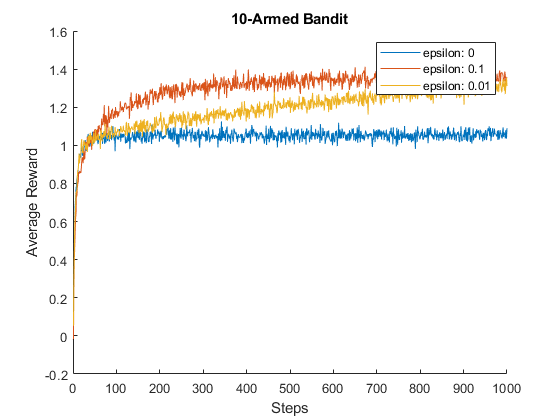
\includegraphics{epsilon_greedy}




\section{Upper-Confidence-Bound}


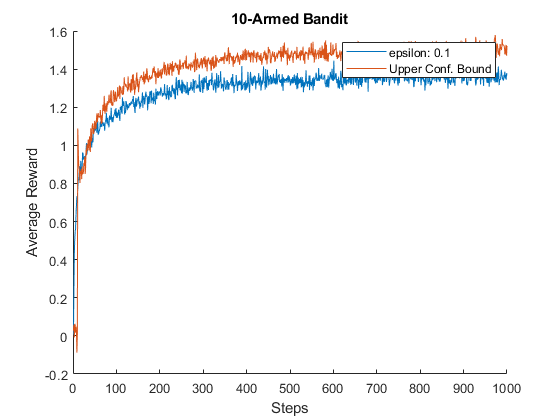
\includegraphics{upper_conf_bound}


\end{document}
